\documentclass{beamer}
\usepackage{ngerman}
\usetheme[pageofpages=of,% String used between the current page and the
                         % total page count.
          bullet=circle,% Use circles instead of squares for bullets.
          titleline=true,% Show a line below the frame title.
          alternativetitlepage=true,% Use the fancy title page.
          %titlepagelogo=chocolategirl,% Logo for the first page.
          %watermark=chocolategirl,% Watermark used in every page.
          watermarkheight=50px,% Height of the watermark.
          watermarkheightmult=4,% The watermark image is 4 times bigger
                                % than watermarkheight.
          ]{Torino}
\usepackage{amsmath}
\usepackage{textcomp}

\usepackage{tikz}						%TikZ graphics
\usepackage{pgfplots}
\pgfplotsset{compat=1.11}
\usepackage{pgfplotstable}

\author{H. Diethelm}
\title{Feldquantisierung}
\date{\today}

\begin{document}
\begin{frame}[t,plain]
\titlepage
\end{frame}

\begin{frame}{Programm}
\tableofcontents
\end{frame}

% ----------------------------------------------------------------------------

\section{Einleitung}
\begin{frame}[t]{Einleitung}
	\vspace*{-0.5cm}
	\begin{center}
			\begin{minipage}{0.35\textwidth}
				\begin{align*}
				\nabla\cdot E &= \frac{\rho}{\varepsilon_0} & \quad
				\nabla\times B &= \mu_0 j  + \mu_0 \varepsilon_0\frac{\partial E}{\partial t}\\
				\nabla\cdot B &=0 & \quad
				\nabla\times E &= -\frac{\partial B }{\partial t}
				\end{align*}
			\end{minipage}
			
			$\Downarrow$
			
			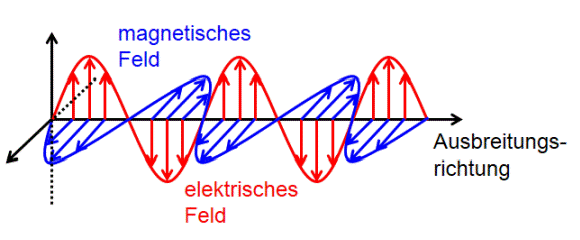
\includegraphics[width=0.35\textwidth]{emwelle.png}

			$\Downarrow$

			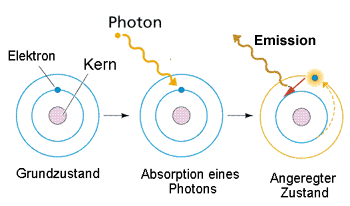
\includegraphics[width=0.35\textwidth]{anregung.png}
	\end{center}

\end{frame}

% ----------------------------------------------------------------------------

\section{Von Maxwell-Gleichungen zu Oszillatoren}
\begin{frame}[t]{Von Maxwell-Gleichungen zu Oszillatoren}
	\vspace*{-0.5cm}
	\begin{center}
		\begin{minipage}{0.35\textwidth}
			\begin{align*}
			\quad(1) &&\nabla\cdot E &= \frac{\rho}{\varepsilon_0} &
			\quad(3) &&\nabla\cdot B &=0 \\
			\quad(2) &&\nabla\times B &= \mu_0 j  + \mu_0 \varepsilon_0\frac{\partial E}{\partial t}&
			\quad(4) && \nabla\times E &= -\frac{\partial B }{\partial t}
			\end{align*}
		\end{minipage}
		
		\vspace*{0.5cm}
		$\Downarrow$
		
		\begin{minipage}{0.35\textwidth}
			\begin{align*}
			\quad(3) && B &= \nabla\times A &
			\quad(1) &&\nabla^2 \varphi - \frac{1}{c^2} \dfrac{\partial^2 \varphi}{\partial t^2} &= -\rho\\
			\quad(4) && E &= -\dfrac{\partial A}{\partial t} - \nabla \varphi &
			\quad(2) && \nabla^2 A - \frac{1}{c^2} \frac{\partial^2 A }{\partial t^2} &= - \mu_0 j
			\end{align*}
		\end{minipage}
	\end{center}
\end{frame}

\begin{frame}[t]{Von Maxwell-Gleichungen zu Oszillatoren}
	\vspace*{-0.5cm}
	\begin{center}
		\begin{minipage}{0.35\textwidth}
			\begin{align*}
			\nabla^2 A - \frac{1}{c^2} \frac{\partial^2 A }{\partial t^2} &= 0
			\end{align*}
		\end{minipage}
		
		\vspace*{0.5cm}
		$\Downarrow$
		
		\begin{minipage}{0.35\textwidth}
			\begin{align*}
			A(x,t) &= \frac{1}{\sqrt{V}} \sum_k \sum_{\alpha=1,2} \left(c_{k,\alpha} \varepsilon^{(\alpha)} e^{i (k \cdot x - \omega_k t)} + \bar{c}_{k,\alpha} \varepsilon^{(\alpha)} e^{-i(k \cdot x - \omega_k t)}\right)\\
			&= \frac{1}{\sqrt{V}} \sum_k \sum_{\alpha=1,2} \left(c_{k,\alpha}(t)u_{k,\alpha}(x) + \bar{c}_{k,\alpha}(t) \bar{u}_{k,\alpha}(x) \right)
			\end{align*}
			\begin{align*}
				c_{k,\alpha}(t) &= c_{k,\alpha} e^{-i \omega_k t} \\
				u_{k,\alpha}(x) &= \varepsilon^{(\alpha)} e^{ik \cdot x}
			\end{align*}
			
		\end{minipage}
	\end{center}
\end{frame}

\begin{frame}[t]{Von Maxwell-Gleichungen zu Oszillatoren}
	\vspace*{-0.5cm}
	\begin{center}
		\begin{minipage}{0.35\textwidth}
			\begin{align*}
			\begin{split}
			H &= \frac{1}{2} \int \left(\frac{1}{\mu_0}|B|^2 + \varepsilon_0|E|^2\right) d^3 x \\
			&= \frac{1}{2} \int \left(c^2 \varepsilon_0 | \nabla\times A |^2 + \varepsilon_0 \left| \dfrac{\partial A}{\partial t} \right|^2 \right) d^3 x \\
			& = \sum_k \sum_{\alpha=1,2} 2 \varepsilon_0 \omega_k^2 \bar{c}_{k,\alpha}(t) c_{k,\alpha}(t)
			\end{split}
			\end{align*}
		\end{minipage}
	\end{center}
\end{frame}

\begin{frame}[t]{Von Maxwell-Gleichungen zu Oszillatoren}
	\vspace*{-0.5cm}
	\begin{center}
		\begin{minipage}{0.35\textwidth}
			\begin{align*}
			& H = \sum_k \sum_{\alpha=1,2} 2 \varepsilon_0 \omega_k^2 \bar{c}_{k,\alpha}(t) c_{k,\alpha}(t) \\
			& Q_{k,\alpha} = \sqrt{\varepsilon_0} \left(c_{k,\alpha}(t) + \bar{c}_{k,\alpha}(t)\right) \quad P_{k,\alpha} = -i \omega_k \sqrt{\varepsilon_0} \left(c_{k,\alpha}(t) - \bar{c}_{k,\alpha}(t)\right) 
			\end{align*}
		\end{minipage}
		
		\vspace*{0.5cm}
		$\Downarrow$
		
		\begin{minipage}{0.35\textwidth}
			\begin{align*}
			H &= \sum_k \sum_{\alpha=1,2} 2 \omega_k^2 
			\underbrace{\left[ \frac{\omega_k Q_{k,\alpha} - i P_{k,\alpha}}{2 \omega_k} \right]}_{\sqrt{\varepsilon_0} \bar{c}_{k,\alpha}(t)}
			\underbrace{\left[ \frac{\omega_k Q_{k,\alpha} + i P_{k,\alpha}}{2 \omega_k} \right]}_{\sqrt{\varepsilon_0} c_{k,\alpha}(t)} \\
			&= \sum_k \sum_{\alpha=1,2} \frac{1}{2} \left(P_{k,\alpha}^2 + \omega_k^2 Q_{k,\alpha}^2\right)
			\end{align*}
		\end{minipage}
		
		Koordinaten und Impulse eines harmonischen Oszillators!
	\end{center}
\end{frame}

% ----------------------------------------------------------------------------

\section{Quantisierung des Wellenfeldes}
\begin{frame}[t]{Quantisierung des Wellenfeldes}
	\vspace*{-0.5cm}
	\begin{center}
		$Q_{k,\alpha}$ und $P_{k,\alpha}$ sind Operatoren $\rightarrow$ $\hat{Q}_{k,\alpha}$ und $\hat{P}_{k,\alpha}$
		
		\begin{minipage}{0.35\textwidth}
			\begin{align*}
			[\hat{Q}_{k,\alpha}, \hat{P}_{k',\alpha'}] &= i \hbar \delta_{kk'}\delta_{aa'} \\
			[\hat{Q}_{k,\alpha}, \hat{Q}_{k',\alpha'}] &= 0 \\
			[\hat{P}_{k,\alpha}, \hat{P}_{k',\alpha'}] &= 0
			\end{align*}
		\end{minipage}
	\end{center}
\end{frame}

\begin{frame}[t]{Quantisierung des Wellenfeldes}
	\vspace*{-0.5cm}
	\begin{center}
		\begin{minipage}{0.35\textwidth}
			\begin{align*}
			a_{k,\alpha} &= \frac{1}{\sqrt{2 \hbar \omega_k}} (\omega_k \hat{Q}_{k,\alpha} + i\hat{P}_{k,\alpha}) \\
			a^+_{k,\alpha} &= \frac{1}{\sqrt{2 \hbar \omega_k}} (\omega_k \hat{Q}_{k,\alpha} - i\hat{P}_{k,\alpha})\\
			\begin{split}
			N_{k,\alpha} &= a^+_{k,\alpha} a_{k,\alpha} = \frac{1}{2 \hbar \omega_k} \left(\hat{P}_{k,\alpha}^2 + \omega_k^2 \hat{Q}_{k,\alpha}^2 + i\omega_k [\hat{Q}_{k,\alpha},\hat{P}_{k,\alpha}] \right) \\
			&= \frac{1}{ \hbar \omega_k } H - \frac{1}{2} = {\cal H} - \frac{1}{2}
			\end{split}
			\end{align*}
		\end{minipage}
	\end{center}
\end{frame}

\begin{frame}[t]{Quantisierung des Wellenfeldes}
	\vspace*{-0.5cm}
	\begin{center}
		\begin{minipage}{0.35\textwidth}
			\begin{align*}
				a_{k,\alpha} &= \frac{1}{\sqrt{2 \hbar \omega_k}} (\omega_k \hat{Q}_{k,\alpha} + i\hat{P}_{k,\alpha}) \\
				a^+_{k,\alpha} &= \frac{1}{\sqrt{2 \hbar \omega_k}} (\omega_k \hat{Q}_{k,\alpha} - i\hat{P}_{k,\alpha})
			\end{align*}
			Die Definition war:
			\begin{align*}
				Q_{k,\alpha} = \sqrt{\varepsilon_0} \left(c_{k,\alpha}(t) + \bar{c}_{k,\alpha}(t)\right) \quad P_{k,\alpha} = -i \omega_k \sqrt{\varepsilon_0} \left(c_{k,\alpha}(t) - \bar{c}_{k,\alpha}(t)\right) 
			\end{align*}
		\end{minipage}
		
		\vspace*{0.5cm}
		$\Downarrow$
		
		\begin{minipage}{0.35\textwidth}
			\begin{align*}
			 c_{k,\alpha} \Rightarrow \sqrt{\frac{\hbar}{2 \varepsilon_0 \omega_k}} a_{k,\alpha} \qquad 
			 \bar{c}_{k,\alpha} \Rightarrow \sqrt{\frac{\hbar}{2 \varepsilon_0 \omega_k}} \, a^+_{k,\alpha}
			\end{align*}
		\end{minipage}
	\end{center}
\end{frame}

\begin{frame}[t]{Quantisierung des Wellenfeldes}
	\vspace*{-0.5cm}
	\begin{center}
		\begin{minipage}{0.35\textwidth}
			\begin{align*}
				N|n\rangle = e_n|n\rangle
			\end{align*}
		\end{minipage}
		
		\vspace*{0.5cm}
		$\Downarrow$
		
		\begin{minipage}{0.35\textwidth}
			\begin{align*}
			Na^+|n\rangle &= (a^+N + a^+)|n\rangle = (e_n + 1)a^+|n\rangle \\
			Na|n\rangle &= (aN - a)|n\rangle = (e_n - 1)a|n\rangle
			\end{align*}
		\end{minipage}
	\end{center}
\end{frame}

\begin{frame}[t]{Quantisierung des Wellenfeldes}
	\vspace*{-0.5cm}
	\begin{center}
		\begin{minipage}{0.35\textwidth}
			\begin{align*}
			a^+|n\rangle &= c_+|n+1\rangle \\
			a|n\rangle &= c_-|n-1\rangle
			\end{align*}
		\end{minipage}
		
		\vspace*{0.5cm}
		$\Downarrow$
		
		\begin{minipage}{0.35\textwidth}
			\begin{align*}
			\begin{split}
			|c_+|^2 &= |c_+|^2 \langle n+1 \, | \, n+1 \rangle = ( a^+ \langle n |\,) \; a^+ \,| n \rangle \\
			&= \langle n |\, a \, a^+ \,|n \rangle = \langle n |\, N + [a,a^+] \,|n \rangle \\
			&= e_n+1
			\end{split}\\
			|c_-|^2 &= 	( a \langle n |\,) \; a \,| n \rangle = \langle n |\, a^+ a \,| n \rangle = e_n
			\end{align*}
		\end{minipage}
		\begin{minipage}{0.35\textwidth}
			\begin{align*}
			a^+\,|n\rangle &= \sqrt{e_n+1}\,|n+1\rangle \\
			a\,|n\rangle &= \sqrt{e_n}\,|n-1\rangle
			\end{align*}
		\end{minipage}
	\end{center}
\end{frame}

\begin{frame}[t]{Quantisierung des Wellenfeldes}
	\vspace*{-0.5cm}
	\begin{center}
		\begin{minipage}{0.35\textwidth}
			\begin{align*}
			e_n \geq 0 \rightarrow n \text{ Integer! }
			\end{align*}
		\end{minipage}
		
		\vspace*{0.5cm}
		$\Downarrow$
		
		\begin{minipage}{0.35\textwidth}
			\begin{align*}
			& a\,|n\rangle = \sqrt{e_n}\,|n-1\rangle  \;, \quad \hdots \; , \quad a\,|2\rangle = \sqrt{2}\,|1\rangle \; , \\
			 & a\,|1\rangle = 0\,|0\rangle \;, \quad a\,|0\rangle = 0\,|0\rangle
			\end{align*}
		\end{minipage}
	\end{center}
\end{frame}

% ----------------------------------------------------------------------------

\section{Photonen}
\begin{frame}[t]{Photonen}
	\vspace*{-0.5cm}
	\begin{center}
		Energiequanten $\rightarrow$ Photonen!
		
		Verhalten wie Elektronen in Potential $\rightarrow$ Teilchen!
		
		\begin{minipage}{0.35\textwidth}
			\begin{align*}
			|0\rangle & \quad \text{kein Feld}\\
			a^+_{k,\alpha}|0\rangle & \quad \text{ein Photon}\\
			\left(1/\sqrt{2}\right)a^+_{k_1,\alpha_1}a^+_{k_2,\alpha_2}|0\rangle & \quad \text{zwei Photonen}
			\end{align*}
		\end{minipage}
		
		\vspace*{0.5cm}
		$\Downarrow$
		
		\begin{minipage}{0.35\textwidth}
			\begin{align*}
			|n_{k_1,\alpha_1}, n_{k_2,\alpha_2}, \, \hdots \, , n_{k_l,\alpha_l}\rangle =
			\prod_{k_i,\alpha_i}\underbrace{\frac{1}{\sqrt{n_{k_i,\alpha_i}}}}_{\text{Normierung}} \underbrace{\left(a^+_{k_i,\alpha_i}\right)^{n_{k_i,\alpha_i}}}_{\text{Aufsteigeoperator}} |0\rangle
			\end{align*}
		\end{minipage}
	\end{center}
\end{frame}

\begin{frame}[t]{Photonen}
	\vspace*{-0.5cm}
	\begin{center}
		
		\begin{minipage}{0.35\textwidth}
			\begin{align*}
			A(x,t) = \frac{1}{\sqrt{V}} \sum_k \sum_{\alpha=1,2} \left(c_{k,\alpha} \varepsilon^{(\alpha)} e^{i (k \cdot x - \omega_k t)} + \bar{c}_{k,\alpha} \varepsilon^{(\alpha)} e^{-i(k \cdot x - \omega_k t)}\right)
			\end{align*}
			\begin{align*}
			c_{k,\alpha} \Rightarrow \sqrt{\frac{\hbar}{2 \varepsilon_0 \omega_k}} a_{k,\alpha} \qquad 
			\bar{c}_{k,\alpha} \Rightarrow \sqrt{\frac{\hbar}{2 \varepsilon_0 \omega_k}} \, a^+_{k,\alpha}
			\end{align*}
		\end{minipage}
		
		\vspace*{0.5cm}
		$\Downarrow$
		
		\begin{minipage}{0.35\textwidth}
			\begin{align*}
			A(x,t) = &\frac{1}{\sqrt{V}} \sum_k \sum_{\alpha=1,2} \sqrt{\frac{\hbar}{2 \varepsilon_0 \omega_k}} \\
			&\left[a_{k,\alpha} \varepsilon^{(\alpha)} e^{i (k \cdot x - \omega_k t)} + a^+_{k,\alpha} \varepsilon^{(\alpha)} e^{-i (k \cdot x - \omega_k t)}\right]
			\end{align*}
		\end{minipage}
		
	\end{center}
\end{frame}

\begin{frame}[t]{Photonen: Feldenergie}
	\vspace*{-0.5cm}
	\begin{center}
		
		\begin{minipage}{0.35\textwidth}
			\begin{align*}
			H = \frac{1}{2} \int \left(\frac{1}{\mu_0} B \cdot B + \varepsilon_0 E \cdot E \right) d^3 x
			\end{align*}
		\end{minipage}
		
		\vspace*{0.5cm}
		$\Downarrow$
		
		\begin{minipage}{0.35\textwidth}
			\begin{align*}
			H &= \frac{1}{2} \sum_k \sum_{\alpha=1,2} \hbar \omega_k \left(a^+_{k,\alpha} a_{k,\alpha} + a_{k,\alpha} a^+_{k,\alpha}\right) \\
			&= \sum_k \sum_{\alpha=1,2} \hbar \omega_k \left(N_{k,\alpha} + \frac{1}{2} \right)
			\end{align*}
			\vspace*{-0.5cm}
			\begin{align*}
			& H|0\rangle = 0 \rightarrow \\
			& H = \sum_k \sum_{\alpha=1,2} \hbar \omega_k N_{k,\alpha}
			\end{align*}
		\end{minipage}
		
	\end{center}
\end{frame}

\begin{frame}[t]{Photonen: Feldenergie}
	\vspace*{-0.5cm}
	\begin{center}
		\begin{minipage}{0.35\textwidth}
			\begin{align*}
				H = \sum_k \sum_{\alpha=1,2} \hbar \omega_k N_{k,\alpha}
			\end{align*}
			\begin{align*}
				N|n\rangle = e_n|n\rangle
			\end{align*}
		\end{minipage}
		
		\vspace*{0.5cm}
		$\Downarrow$
		
		\begin{minipage}{0.35\textwidth}
			\begin{align*}
				H |n_{k_1,\alpha_1}, n_{k_2,\alpha_2}, \, \hdots\rangle = \sum_i \hbar \omega_k n_{k_i,\alpha_i} |n_{k_1,\alpha_1}, n_{k_2,\alpha_2}, \, \hdots\rangle
			\end{align*}
		\end{minipage}
		
	\end{center}
\end{frame}

% ----------------------------------------------------------------------------

\section{Wechselwirkung zwischen Photonen und Elektronen}
\begin{frame}[t]{Wechselwirkung zwischen Photonen und Elektronen}
	\vspace*{-0.5cm}
	\begin{center}
		\begin{itemize}
			\item Keine Wechselwirkung mit Protonen und Neutronen im Kern
			\item Spin vernachl"assigt da kaum Einfluss
		\end{itemize}
	\end{center}
\end{frame}

\begin{frame}[t]{Wechselwirkung zwischen Photonen und Elektronen}
	\vspace*{-0.5cm}
	\begin{center}
		
		\begin{minipage}{0.35\textwidth}
			\begin{align*}
			H = \frac{1}{2m}p^2 + V(x)
			\end{align*}
		\end{minipage}
		
		\vspace*{0.5cm}
		
		$p \rightarrow p-eA$
		
		\begin{minipage}{0.35\textwidth}
			\begin{align*}
			H &= \frac{1}{2m}(p - eA)^2 + V(x)\\
			&= \underbrace{\frac{1}{2m}p^2 + V(x)}_{H_0} + \\
			 & \quad \underbrace{\frac{1}{2m}\left[- e p \cdot A(x, t) - e A(x, t) \cdot p + e^2 A(x, t) \cdot A(x, t) \right]}_{H_{\text{int}}}
			\end{align*}
		\end{minipage}
	\end{center}
\end{frame}

\begin{frame}[t]{Wechselwirkung zwischen Photonen und Elektronen}
	\vspace*{-0.5cm}
	\begin{center}
		
		\begin{minipage}{0.35\textwidth}
			\begin{align*}
			H_{\text{int}} = \frac{1}{2m}\left[- e p \cdot A(x, t) - e A(x, t) \cdot p + e^2 A(x, t) \cdot A(x, t) \right]
			\end{align*}
		\end{minipage}
		
		\vspace*{0.5cm}
		
		$\nabla \cdot A = 0$ $\rightarrow$ $p \cdot A(x, t)$ vertauschen
				
		$\Downarrow$
		
		\begin{minipage}{0.35\textwidth}
			\begin{align*}
				H_{\text{int}} = -\frac{e}{m} A(x, t) \cdot p + \frac{e^2}{2m}A(x, t) \cdot A(x, t)
			\end{align*}
		\end{minipage}
	\end{center}
\end{frame}

\begin{frame}[t]{Wechselwirkung zwischen Photonen und Elektronen}
	\begin{center}
		
		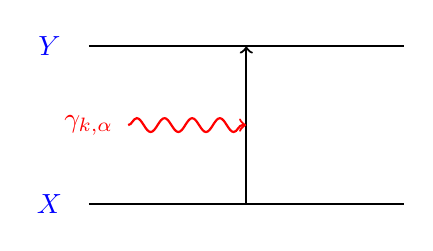
\begin{tikzpicture}

			\node[color=blue] at (0, 0) {$X$};	
			\node[color=blue] at (0, 2) {$Y$};
			\node[color=red] at (0.5, 1) {$\gamma_{k,\alpha}$};
			
			\draw[color=black,thick] (0.5, 0) -- +( 4, 0);
			\draw[color=black,thick] (0.5, 2) -- +( 4, 0);
			\draw[->,color=black,thick] (2.5, 0) -- +( 0, 2);	
			\draw[->,decorate, decoration={snake},color=red,thick] (1, 1) -- +( 1.5, 0);
			
		\end{tikzpicture}

		$X \rightarrow Y$
		
		\begin{minipage}{0.35\textwidth}
			\begin{align*}
			\langle Y| \, H \, |X \rangle = \langle Y| \, H_0 + H_{\text{int}} \, |X \rangle = \underbrace{\langle Y| \, H_0 \, |X \rangle}_{=0} + \langle Y| \, H_{\text{int}} \, |X \rangle
			\end{align*}
		\end{minipage}
		
		\vspace*{0.5cm}
		$\Rightarrow$ nur $H_{\text{int}}$ betrachten!
		
	\end{center}
\end{frame}

\begin{frame}[t]{Wechselwirkung zwischen Photonen und Elektronen}
	\begin{center}
		Absorption $X \rightarrow Y$\\
		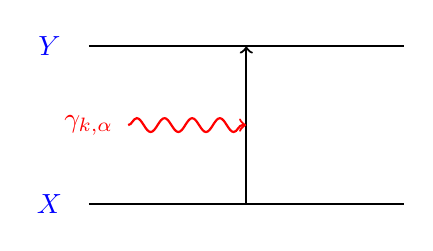
\begin{tikzpicture}
			\node[color=blue] at (0, 0) {$X$};	
			\node[color=blue] at (0, 2) {$Y$};
			\node[color=red] at (0.5, 1) {$\gamma_{k,\alpha}$};
			
			\draw[color=black,thick] (0.5, 0) -- +( 4, 0);
			\draw[color=black,thick] (0.5, 2) -- +( 4, 0);
			\draw[->,color=black,thick] (2.5, 0) -- +( 0, 2);	
			\draw[->,decorate, decoration={snake},color=red,thick] (1, 1) -- +( 1.5, 0);
		\end{tikzpicture}
		
		\begin{minipage}{0.35\textwidth}
			\begin{align*}
			&\langle Y; n_{k,\alpha} - 1 |\, H_{\text{int}} \,| X; n_{k,\alpha} \rangle = \\
			&-\frac{e}{m} \left\langle Y; n_{k,\alpha} - 1 \biggl| 
			\, \frac{1}{\sqrt{V}} \sqrt{\frac{\hbar}{2 \varepsilon_0 \omega_k}}a_{k,\alpha} \varepsilon^{(\alpha)} e^{i(k \cdot x-\omega_k t)} \cdot p \,
			\biggl| X; n_{k,\alpha} \right\rangle\\
			&= -\frac{e}{m} \sqrt{\frac{n_{k,\alpha} \hbar}{2 \varepsilon_0 \omega_k V}} \left\langle Y \left|
			\, e^{ik \cdot x} \varepsilon^{(\alpha)} \cdot p \,
			\right| X \right\rangle e^{-i\omega_k t}
			\end{align*}
		\end{minipage}
		
	\end{center}
\end{frame}

\begin{frame}[t]{Wechselwirkung zwischen Photonen und Elektronen}
	\begin{center}
		Spontane Emission $X \rightarrow Y$ \quad Stimulierte Emission $X \rightarrow Y$\\
		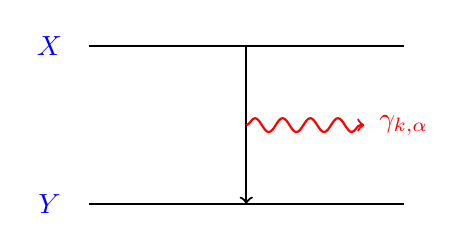
\begin{tikzpicture}
		\node[color=blue] at (0, 0) {$Y$};	
		\node[color=blue] at (0, 2) {$X$};
		\node[color=red] at (4.5, 1) {$\gamma_{k,\alpha}$};
		
		\draw[color=black,thick] (0.5, 0) -- +( 4, 0);
		\draw[color=black,thick] (0.5, 2) -- +( 4, 0);
		\draw[->,color=black,thick] (2.5, 2) -- +( 0, -2);	
		\draw[->,decorate, decoration={snake},color=red,thick] (2.5, 1) -- +( 1.5, 0);
		\end{tikzpicture}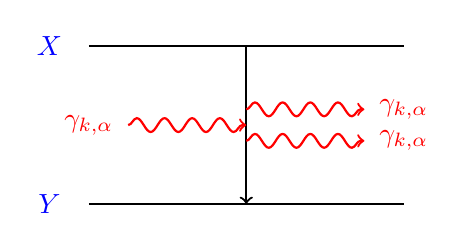
\begin{tikzpicture}
		\node[color=blue] at (0, 0) {$Y$};	
		\node[color=blue] at (0, 2) {$X$};
		\node[color=red] at (0.5, 1) {$\gamma_{k,\alpha}$};
		\node[color=red] at (4.5, 0.8) {$\gamma_{k,\alpha}$};
		\node[color=red] at (4.5, 1.2) {$\gamma_{k,\alpha}$};
		
		\draw[color=black,thick] (0.5, 0) -- +( 4, 0);
		\draw[color=black,thick] (0.5, 2) -- +( 4, 0);
		\draw[->,color=black,thick] (2.5, 2) -- +( 0, -2);
		\draw[->,decorate, decoration={snake},color=red,thick] (1, 1) -- +( 1.5, 0);
		\draw[->,decorate, decoration={snake},color=red,thick] (2.5, 0.8) -- +( 1.5, 0);
		\draw[->,decorate, decoration={snake},color=red,thick] (2.5, 1.2) -- +( 1.5, 0);
		\end{tikzpicture}
		
		\begin{minipage}{0.35\textwidth}
			\begin{align*}
			&\langle Y; n_{k,\alpha} + 1 |\, H_{\text{int}} \,| X; n_{k,\alpha} \rangle = \\
			&-\frac{e}{m} \left\langle Y; n_{k,\alpha} + 1 \biggl| 
			\, \frac{1}{\sqrt{V}} \sqrt{\frac{\hbar}{2 \varepsilon_0 \omega_k}}a^+_{k,\alpha} \varepsilon^{(\alpha)} e^{-i(k \cdot x-\omega_k t)} \cdot p \,
			\biggl| X; n_{k,\alpha} \right\rangle\\
			&= -\frac{e}{m} \sqrt{\frac{ (n_{k,\alpha}+1) \hbar}{2 \varepsilon_0 \omega_k V}} \left\langle Y \left| 
			\, e^{-ik \cdot x} \varepsilon^{(\alpha)} \cdot p \,
			\right| X \right\rangle e^{i\omega_k t}
			\end{align*}
		\end{minipage}
		
	\end{center}
\end{frame}

\begin{frame}[t]{Einsteinkoeffizienten}
	\begin{center}
		\vspace*{-0.2cm}
		$| \langle Y| \, H_{\text{int}} \, |X \rangle |^2$
		\vspace*{0.2cm}
		
		Spontane Emission $X \rightarrow Y$ \quad Stimulierte Emission $X \rightarrow Y$\\
		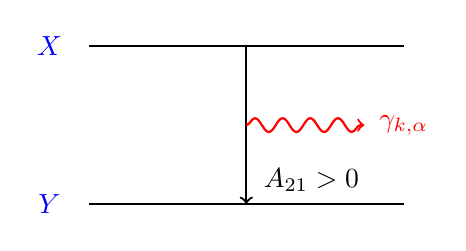
\begin{tikzpicture}
		\node[color=blue] at (0, 0) {$Y$};	
		\node[color=blue] at (0, 2) {$X$};
		\node[color=red] at (4.5, 1) {$\gamma_{k,\alpha}$};
		\node[color=black,anchor=west] at (2.6, 0.3) {$A_{21} > 0$};
		
		\draw[color=black,thick] (0.5, 0) -- +( 4, 0);
		\draw[color=black,thick] (0.5, 2) -- +( 4, 0);
		\draw[->,color=black,thick] (2.5, 2) -- +( 0, -2);	
		\draw[->,decorate, decoration={snake},color=red,thick] (2.5, 1) -- +( 1.5, 0);
		\end{tikzpicture}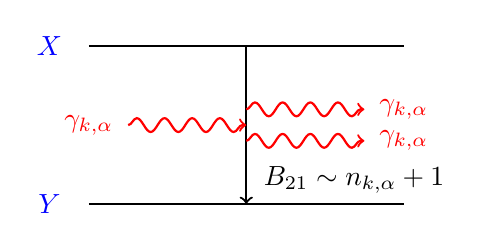
\begin{tikzpicture}
		\node[color=blue] at (0, 0) {$Y$};	
		\node[color=blue] at (0, 2) {$X$};
		\node[color=red] at (0.5, 1) {$\gamma_{k,\alpha}$};
		\node[color=red] at (4.5, 0.8) {$\gamma_{k,\alpha}$};
		\node[color=red] at (4.5, 1.2) {$\gamma_{k,\alpha}$};
		\node[color=black,anchor=west] at (2.6, 0.3) {$B_{21} \sim n_{k,\alpha} + 1$};
		
		\draw[color=black,thick] (0.5, 0) -- +( 4, 0);
		\draw[color=black,thick] (0.5, 2) -- +( 4, 0);
		\draw[->,color=black,thick] (2.5, 2) -- +( 0, -2);
		\draw[->,decorate, decoration={snake},color=red,thick] (1, 1) -- +( 1.5, 0);
		\draw[->,decorate, decoration={snake},color=red,thick] (2.5, 0.8) -- +( 1.5, 0);
		\draw[->,decorate, decoration={snake},color=red,thick] (2.5, 1.2) -- +( 1.5, 0);
		\end{tikzpicture}
		
		Absorption $X \rightarrow Y$\\
		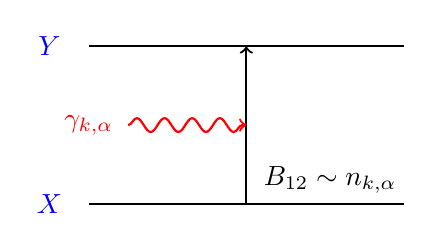
\begin{tikzpicture}
		\node[color=blue] at (0, 0) {$X$};	
		\node[color=blue] at (0, 2) {$Y$};
		\node[color=red] at (0.5, 1) {$\gamma_{k,\alpha}$};
		\node[color=black,anchor=west] at (2.6, 0.3) {$B_{12} \sim n_{k,\alpha}$};
		
		\draw[color=black,thick] (0.5, 0) -- +( 4, 0);
		\draw[color=black,thick] (0.5, 2) -- +( 4, 0);
		\draw[->,color=black,thick] (2.5, 0) -- +( 0, 2);	
		\draw[->,decorate, decoration={snake},color=red,thick] (1, 1) -- +( 1.5, 0);
		\end{tikzpicture}
		
	\end{center}
\end{frame}

\begin{frame}
\centering 
\huge{Vielen Dank f"ur Ihre Aufmerksamkeit!} \\
\huge{Fragen?}\\

\includegraphics[width=0.2\textwidth]{questionguy.png}


\end{frame}


\end{document}

